\section{Seismic Migration}

The purpose of the \emph{seismic exploration} is to understand the
constitution of the interior earth as much as possible. As we know, it is
impractical or even impossible to penetrate the earth and put your camera
there to capture the image, other indirect approaches are used to attain
the similar or same result. These approaches includes seismological
measurement, electromagnetic measurement and gravity measurement. As these
approaches are indirect, they usually give a analyze or indication of the
measured result. Some tools, such as computers, are required as part of the
analyze and the capability of the tools may be the bottleneck of the
analyze. For example, in the past, with the poor computational performance
of the computer, the data in only a small region and in a low resolution
could the seismologists analyzed due to the limited computing power.

As the Moore's Law indicates that the number of transistors double every 18
months, the computer gains much more computing power than before. Some
seismological method, which are computationally-demanding, seems not
practical in the past, can be implemented by utilizing the advanced
technology today. One of the most useful but computationally-demanding
algorithm, Reverse Time Migration algorithm, also comes into reality.

Reverse Time Migration is an algorithm of seismic migration. And seismic
migration is one of the most important part of seismic exploration, and
more specifically, seismic imaging. By seismic migration, the constitution
of the interior earth could be imaged, sketching, for example, the water,
rocks, gas, oil, faults etc in the subsurface.

\subsection{General Process of Seismic Exploration}

Seismic exploration, as one of the background knowledge of this thesis,
is explained in this section. Figure (\ref{fig:sea_floor_seismic}) shows a
typical scenario of a marine
based seismic exploration. The vessel will inject waves periodically by the
air gun. The waves just injected will spread in all direction quickly until
it penetrate different media, such as rocks, ands, gas, or oil beneath the
water, where the waves will reflect back or refract through another medium.
The reflected waves, or those refracts first, then reflected waves would be
recorded by an large array of Geo phones. In figure
(\ref{fig:sea_floor_seismic}), another smaller ship shows up, dragging a
cable
which contains an array of sensors to record the reflected signals.

\begin{figure}
  \centering
  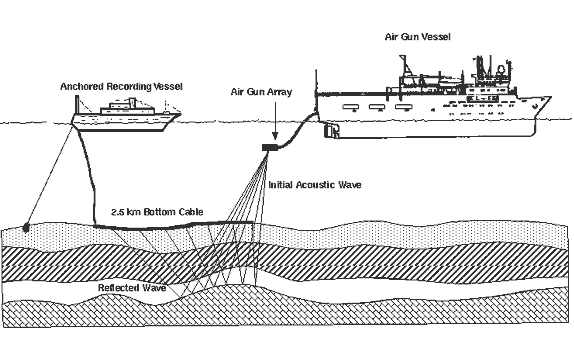
\includegraphics[scale=0.5]{img/Seafloor_Seismic.png}
  \caption{Marine-based Seismic Exploration}
  \label{fig:sea_floor_seismic}
\end{figure}

Geophysics data processing then follows the process of recording the
signals. First of all, multiple steps should be applied to perform the
preprocessing. For example, use the bandpass filter to remove the noise.
And last of all, is the migration step to reconstruct the image of
subsurface.

The detail of how the data are processed is not the topic of this thesis,
so I won't explain it too much. Those who are interested in the subject can
find more information with the help of the search engine. In this thesis, I
only concern about what is relevant with the FPGA implementation of the
computational part, which is explained in next subsection.

\subsection{Reverse Time Migration}

In this subsection, I present a general introduction for Reverse Time
Migration with some seismic terminologies. Revere Time Migration use the
source and recorded signals as input, following a series of computing, then
produce an image of the velocity model, which can maps to the real image of
the interior earth.

You may wonder why the velocity can be mapped to the real constitution of
the interior earth. There are several different objects inside the earth,
such as water, rocks, salt, gas, oil and they are the medium while the wave
propagating through them. The speed of the wave, usually the acoustic wave,
varies from the different medium, for example, the speed of sound is nearly
340 meter per second at temperature 20 degree. If we can generate a model
of the speed inside the earth, we can infer what is inside the earth.

The conventional one-way pre-stack depth migration approach, works well in
the layer medium, shown in Figure (\ref{fig:layer_structure}). If the desired
layer, such as the gas or the oil lies horizontally, it can be easily
discovered with the conventional approach.

\begin{figure}[h]
  \centering
  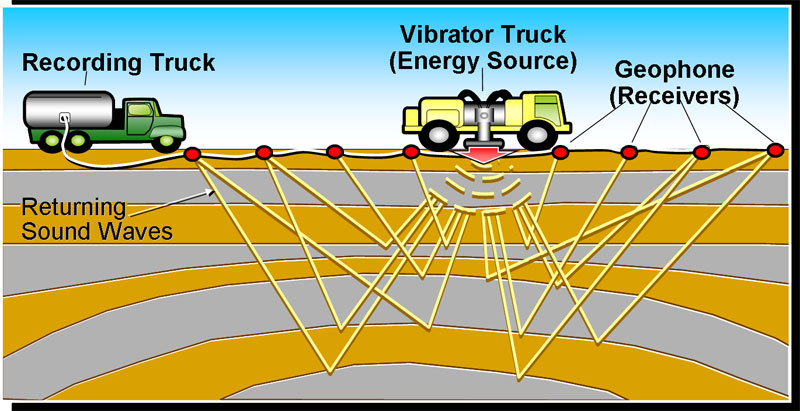
\includegraphics[scale=.45]{img/layer_structure.jpg}
  \caption{Layered structure of the interior earth}
  \label{fig:layer_structure}
\end{figure}

However, not all desired resources are exposed in such a friendly form.
There may be some hill or large rocks beneath the sea, which will obstruct
the desired resource. In addition, some resources will stay in vertical
form or other forms instead of the restrict horizontal form. The
conventional one-way pre-stack depth migration approach could not handle
the previous situation. Thus why Reverse Time Migration emerged.

Reverse Time Migration algorithm is not a new algorithm, instead, it is
first put forward in the 1970s. However, people at that time thinks that it
is impractical or impossible to use such algorithm in practice due to the
tensive  computation requirement. But nowadays, it is impossible to
implement the Reverse Time Migration thanks to the fast developing of
computers.

Instead of just one-way pre-stack depth migration, the Reverse Time
Migration is a two-way pre-stack depth migration, which handles steeply
dipping events, turning waves and multiples. The detail of the algorithm
will be explained in the next section.

Figure (\ref{fig:comparison}) show an introductory example with synthetic
data that illustrates the potential power of the Reverse Time Migration.
There are mainly two part of object in the model, one is water (color from
blue to yellow), the other one is salt (color in red). The figure in the
left is not a real image of the interior earth, but a velocity of that
zone. As the water gets deeper, the speed of the sound becomes faster, so
that is why the color turns from blue to yellow and dark yellow. The salt
is solid object, where the speed of sound is much faster than that in the
water, so the color is in red, a darker color than yellow.

\begin{figure}[h]
  \hfill
  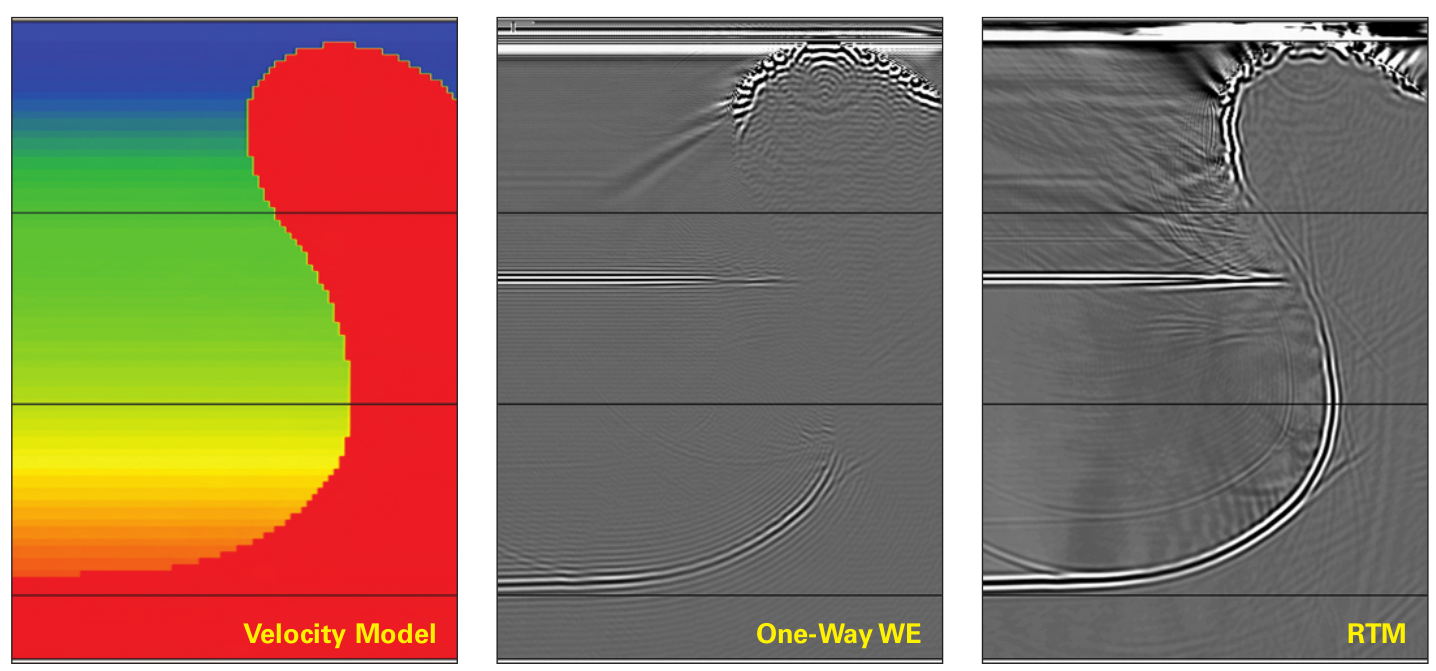
\includegraphics[scale=.25]{img/velocity_model.png}
  \caption{Synthetic comparison of salt flank}
  \label{fig:comparison}
\end{figure}

Concerning about the result, we take a comparison of the middle and right
one in Figure (\ref{fig:comparison}). The middle one is generated using the
one-way wave equation. It is obvious that the salt flank below the overhang
is poorly imaged. On real data, it is difficult to understand the dip and
the structure of sedimentary strata in similar overhang zone. Thus the
potential existence of gas or oil against the salt are impossible to
identify. On the other hand, the last figure, which is produced using the
RTM algorithm, yielding a big improvement. It has a clear profile that is
similar to the original synthetic data.
